\normaltrue
\correctiontrue

%\UPSTIidClasse{11} % 11 sup, 12 spé
%\newcommand{\UPSTIidClasse}{12}

\exer{Mouvement T -- $\star$ \label{CIN:02:B2:13:01:02}}
\setcounter{question}{0}\marginnote{\xpComp{CIN}{02}}%\marginnote{\UPSTIcompetence[2]{B2-13}}
\index{Compétence B2-13}\index{Compétence CIN-02}
\index{Mécanisme à 1 translation}
\ifcorrection
\else
\marginote{\marginnote{\textbf{Pas de corrigé pour cet exercice.}}}
\fi

\ifprof
\else ~\\
Soit le mécanisme de la figure \ref{fig_01_T_02:01_T_01}. On note $\vect{AB}=\lambda(t)\vect{i_0}$.
\begin{marginfigure}
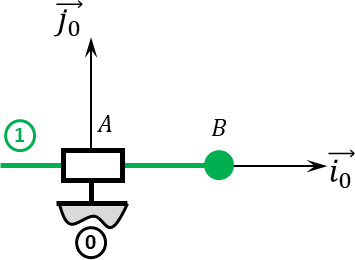
\includegraphics[width=\linewidth]{01_T_01}
\caption{\label{fig_01_T_02:01_T_01} 1 translation}
\end{marginfigure}
\fi

\question{Donner le torseur cinématique $\torseurcin{V}{1}{0}$ au point $B$.}
\ifprof ~\\
$\torseurcin{V}{1}{0} = \torseurl{\vect{0}}{\dot{\lambda}(t)\vi{0}}{\forall P}$.

$\vectv{B}{1}{0} = \deriv{\vect{AB}}{\rep{0}}=\dot{\lambda}(t)\vi{0}$.
\else
\fi

\question{Déterminer $\vectg{B}{1}{0}$.}
\ifprof  ~\\
 $\vectg{B}{1}{0} = \deriv{\vectv{B}{1}{0}}{\rep{0}}=\ddot{\lambda}(t)\vi{0}$.
\else
\fi


\ifprof
\else
\marginnote{
\begin{solution}
\begin{enumerate}
\item $\torseurcin{V}{1}{0} = \torseurl{\vect{0}}{\dot{\lambda}(t)\vi{0}}{\forall P}$.
\item  $\vectg{B}{1}{0} =\ddot{\lambda}(t)\vi{0}$.
\end{enumerate} 
\end{solution}}

\marginnote{Corrigé  voir \ref{CIN:02:B2:13:01:02}.}
\fi


